\documentclass[
	a4paper,
	parskip
]{scrartcl}

\usepackage[english]{babel}
\usepackage{authblk}
\usepackage{amsthm}
\usepackage{amsmath}
\usepackage{amssymb}
\usepackage{booktabs}
\usepackage{float}
\usepackage{multirow}
\usepackage{physics}
\usepackage{siunitx}
\usepackage{hyperref}
\usepackage{cleveref}
\usepackage{subcaption}
\usepackage{pgfplots}
\usepackage[
  backend=biber,
  sorting=none
]{biblatex}
\usepackage[american]{circuitikz}
\usepackage{glossaries}

\addbibresource{literature.bib}

\makeglossaries
\newglossaryentry{s5990}{name=S5990, description={Hamamatsu two-dimensional PSD}}
\newacronym{psd}{PSD}{position-sensitive detector}
\newacronym{gbp}{GBP}{gain-bandwidth-product}

\title{Position-sensitive device}
\author{Bodo Kaiser}
\affil{Ludwig-Maximilians-Universität München}
\affil{\textit{bodo.kaiser@physik.uni-muenchen.de}}

\begin{document}

\maketitle
\tableofcontents

\section{Introduction}

We define a position-sensitive device as a device that outputs voltages proportional to the center of mass coordinates of a light beam incident on a sensitive area.

The present document summarizes the insights acquired on the journey of building such a device.

\subsection{Motivation}

Position-sensitive devices are used in a wide range of industrial and commercial applications, including displacement sensing and beam alignment, see Ref.~\cite[p.~22]{Maekynen00}.

We are interested in using a position-sensitive device for beam pointing alignment in our quantum optics laboratory.

The beam pointing refers to a laser beam's spatial focus and can change through thermal and mechanical effects.
Uncompensated changes in beam alignment can quickly degrade the overall performance of an optical system.
Therefore, it is crucial to align the beam pointing to ensure the optical system's proper operation at hand.

\subsection{Overview}

This document is organized as follows.

The first two sections introduce the theory of the (position-sensitive) photodiode and the operational amplifier.
These sections are rather elaborate and should be skipped by the pragmatic scientist.

The third section describes the (electrical) schematics of the detector.
If you want to adjust parameters, e.g., gain or bandwidth, you should read these sections.

The fourth section is the only significant section if you want to build a \gls{psd}.
If you also want an example of using the \gls{psd} in an optical setup to determine the spatial resolution, you should also read the fifth section.
Finally, the appendix gives some guidance on troubleshooting.

\subsection{Requirements}

The requirements are specified rather loose. The only hard requirement concerns the connectors and voltages of the power supply. The power connector should be a LEMO4 whose pin configuration is compatible with the \SI{\pm15}{\volt} dual-voltage power supplies used in the labs. Features that would be nice to have are:
\begin{enumerate}
	\item The device should be sensible with optical powers that are safe to operate, i.e., $P<\SI{1}{\micro\watt}$. There is no preferred wavelength.
	\item For easy integration into existing optical setups, the device should be as compact as possible. Additional space, if needed, should be occupied by elonging the height. The sensitive area of the detector should be on the bottom. The connectors should be on the top to avoid cables blocking the beam path.
	\item It should be possible to mount different detector sizes on the device.
\end{enumerate}
The range of the output voltages of the device can be chosen for the optimal signal-to-noise ratio.

\subsection{Specification}

\begin{figure}[H]
	\centering
	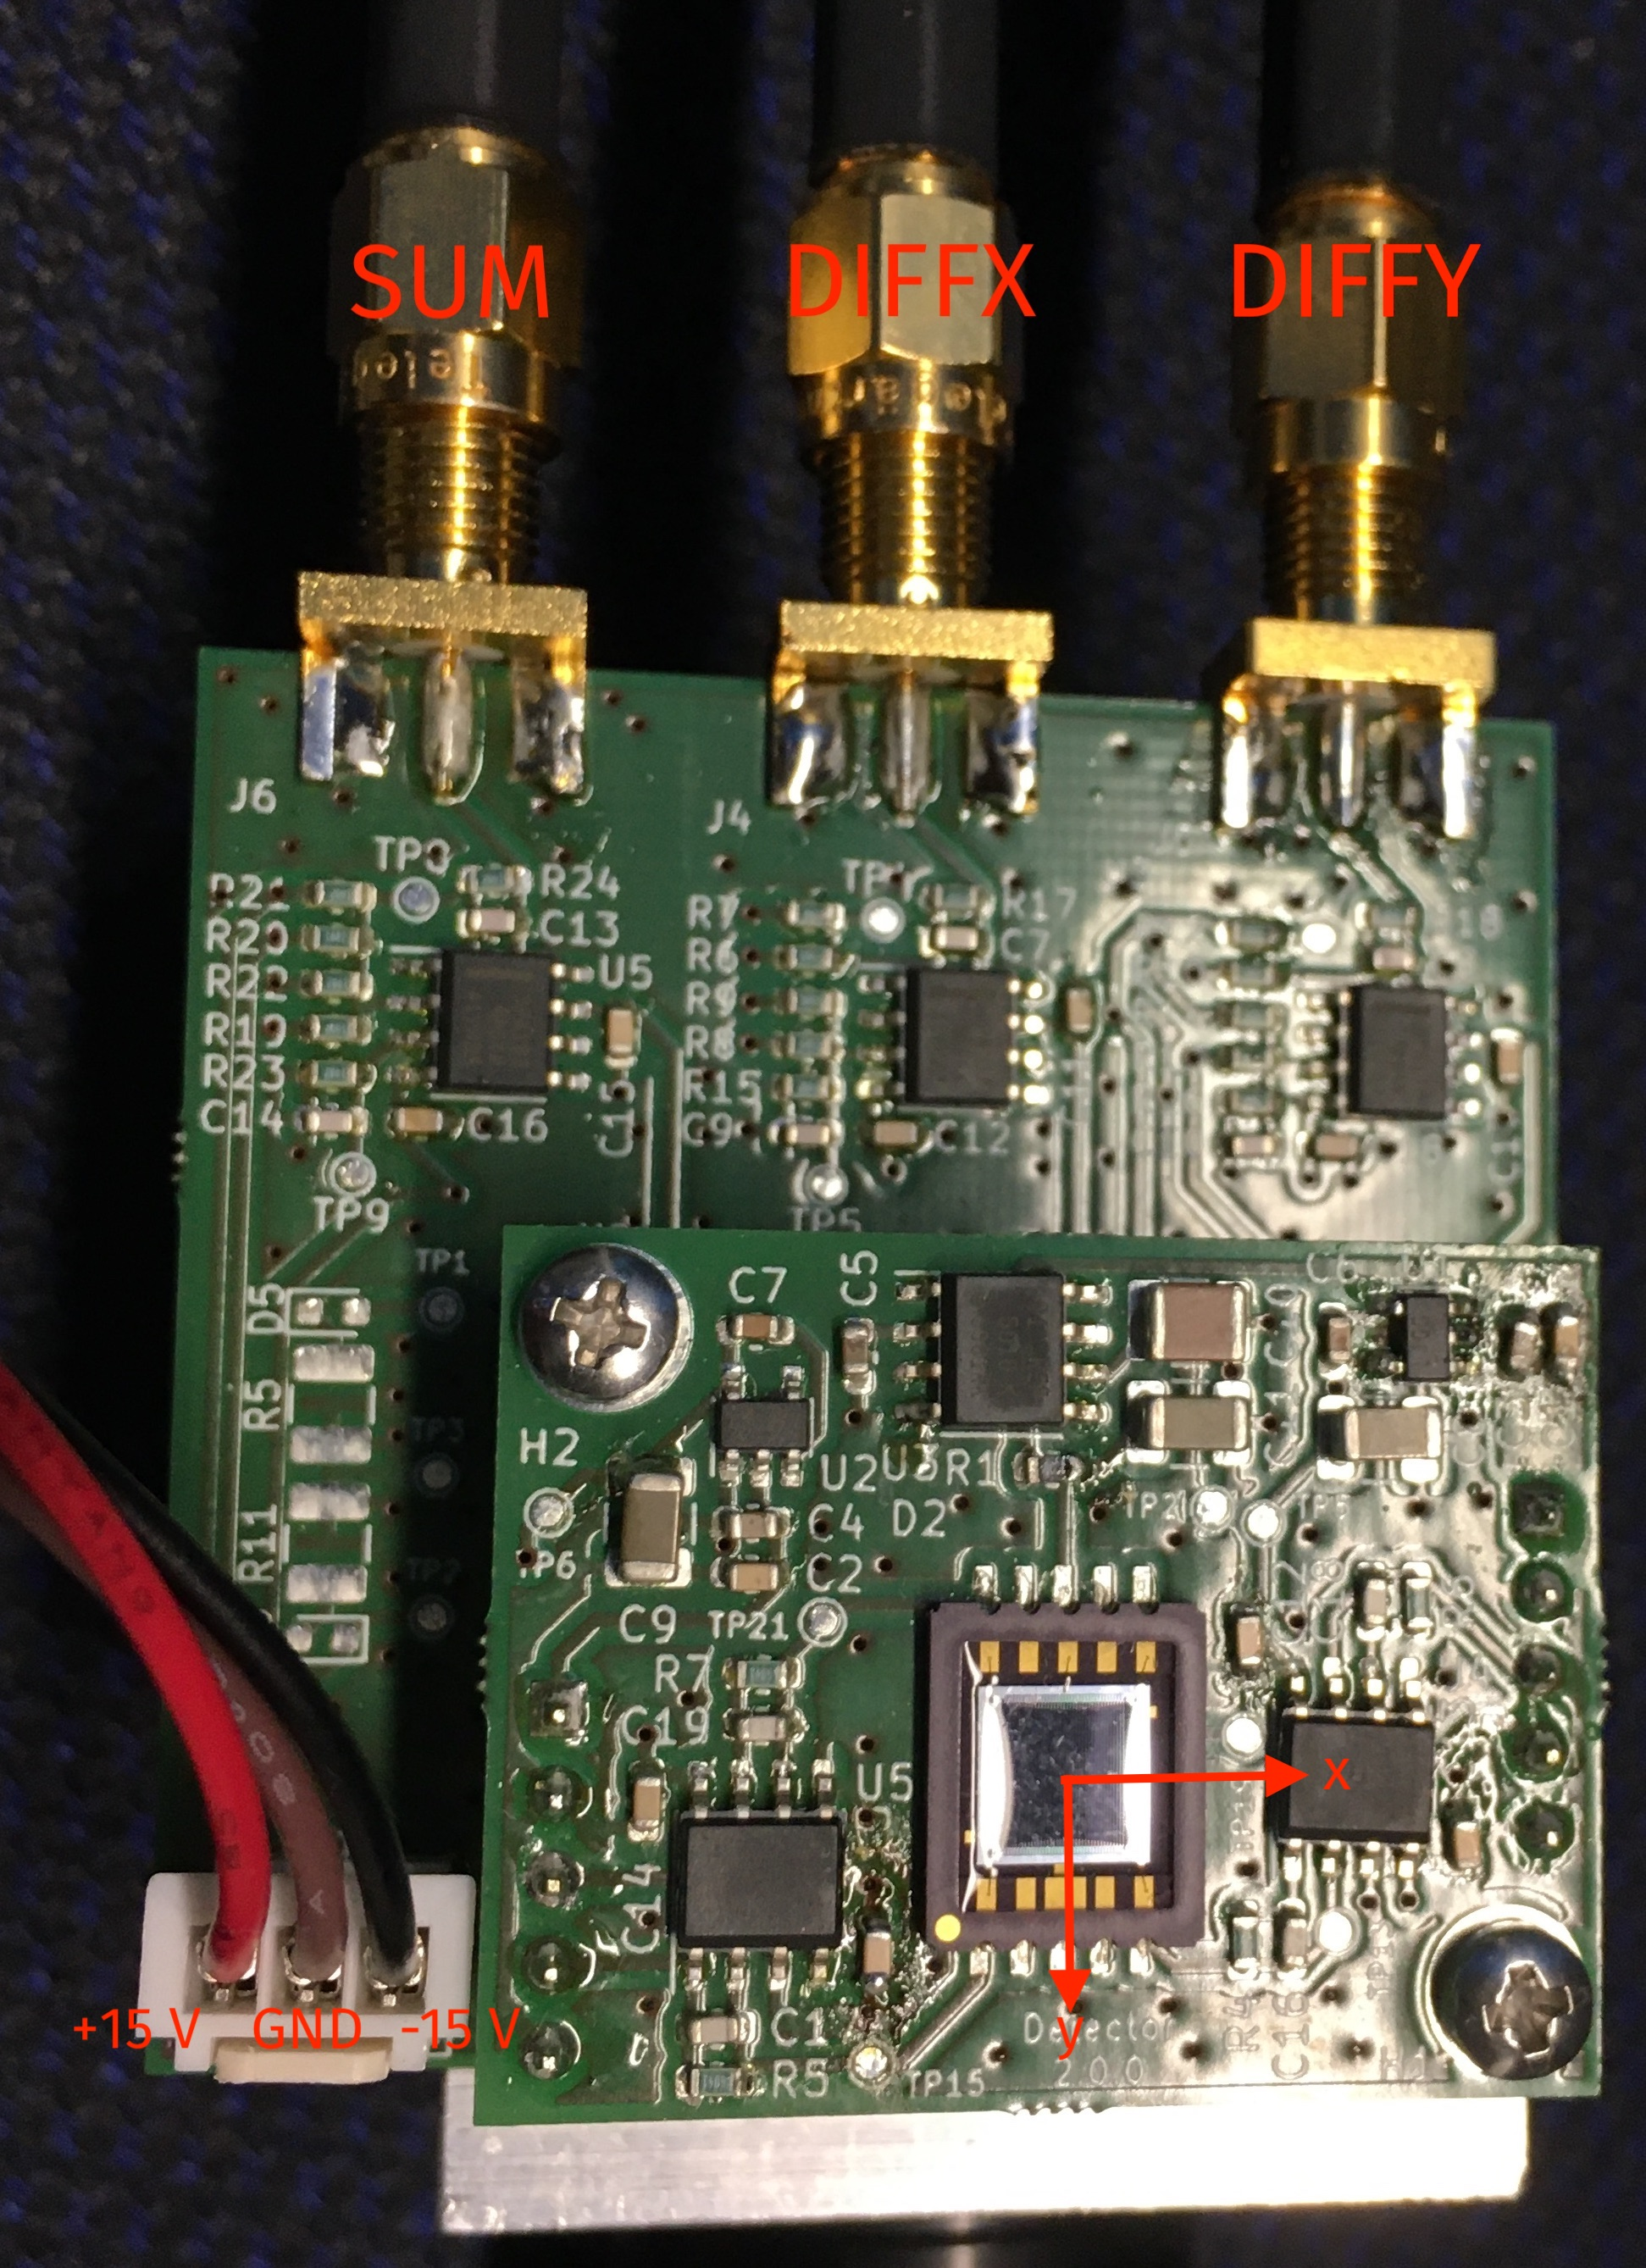
\includegraphics[scale=0.2]{detector.jpg}
	\caption{\gls{psd} on optical mount with connected cables}\label{fig:detector}
\end{figure}
\Cref{fig:detector} shows an image of the \gls{psd}.
The output voltage signals can be tapped from the upper \gls{sma} connectors.
The upper left connector gives the SUM voltage which reflects the total intensity of the optical signal.
The upper center connector gives the DIFFX voltage which reflects the difference proportional to the horizontal position on the sensitive area.
The upper right connector gives the DIFFY voltage which is proportional to the vertical position.
The SUM voltage is required to normalize the difference signals.
The DIFFX voltage increases when moving the light beam on the sensitive area to the right while the DIFFY voltage increases while moving the light beam to the bottom.
The device is powered by a 3-pin connector.
The outer (left) cable is the positive \SI{+15}{\volt} supply while the opposite cable is negative \SI{-15}{\volt} supply.
The center cable of the 3-pin connector has to reference ground.
The power connector has no polarity protection so be careful!

\begin{table}[htb]
  \centering
  \begin{tabular}{lcccc}
    \toprule
      Parameter & Minimum & Typical & Maximum \\
    \midrule
      Output voltages & \SI{-13}{\volt} & \SIrange{-2}{+2}{\volt} & \SI{+13}{\volt} \\
      Supply voltages & \SI{\pm13}{\volt} & \SI{\pm15}{\volt} & \SI{\pm37}{\volt} \\
      Spatial resolution & \SI{5.0}{\micro\meter} & \SI{2}{\micro\meter} & \SI{1}{\micro\meter} \\
      Bandwidth & & \SI{1400}{\kilo\hertz} & \\
    \bottomrule
  \end{tabular}
  \captionsetup{width=.8\textwidth}
  \caption{Specifications of the presented \gls{psd}}\label{tab:specifications}
\end{table}
\Cref{tab:specifications} summarizes the specifications of the presented \gls{psd}.
These specifications are only a rough estimate and we only assembled one \gls{psd} so far.
\section{Requirements}

\begin{enumerate}
    \item Dual power supply $V_\pm=\pm\SI{15}{\volt}$
    \item Ethernet network interface
    \item Spatial resolution $\Delta x=\SI{1}{\micro\meter}$
\end{enumerate}
\section{Position-sensitive detector}

% TODO: overview of position-sensitive detectors and why we choose the lateral pin-cushion type

% TODO: specify pages \cite{Noorlag74}

% TODO: diagram of depletion region for lateral photodiode
% TODO: motivate value for reverse bias
% TODO: diode leakage current
% TODO: noise model
% TODO: responsitivity
% TODO: bandwidth limit
% TODO: photon shot noise

\begin{figure}[H]
	\centering
	\begin{circuitikz}
		\draw (0, 0) node[circ]{};
		\draw (+2, +2) node[ocirc, label=X1]{} to[photodiode] (0, 0);
		\draw (-2, -2) node[ocirc, label=X2]{} to[photodiode] (0, 0);
		\draw (+2, -2) node[ocirc, label=Y2]{} to[photodiode] (0, 0);
		\draw (-2, +2) node[ocirc, label=Y1]{} to[photodiode] (0, 0);
		\draw (0, 0) -- ++(0, -2.5) node[ocirc, label=Cathode, rotate=180]{};
	\end{circuitikz}
	\caption{Position-sensitive detector as photodiodes}
\end{figure}

% TODO: mention non-linearity of voltage response to illumination

\begin{figure}[H]
	\centering
	\begin{circuitikz}
		\draw (-3, -2) to[current source, l=$I_\text{photo}$] ++(0, 4);
		\draw (-1, -2) node[circ]{} to[current source, l=$I_\text{dark}$] ++(0, 4) node[circ]{};
		\draw (1, -2) node[circ]{} to[resistor, l=$R_d$] ++(0, 4) node[circ]{};
		\draw (3, -2) to[capacitor, l=$C_d$] ++(0, 4);
		\draw (-3, -2) -- ++(6, 0);
		\draw (-3, 2) -- ++(6, 0);
		\draw (0, -2) -- ++(0, -1) node[ocirc, label=Cathode, rotate=180]{};
		\draw (0, 2) -- ++(0, 1) node[ocirc, label=Anode]{};
	\end{circuitikz}
	\caption{Photodiode equivalent circuit}
\end{figure}

\begin{equation}
	I_\text{leakage}=I_\text{dark}\left(1-e^{\frac{qV_d}{k_BT}}\right)
\end{equation}
\section{Preamplifier}

The photocurrents created by our detector are in the range of microampere where they are vulnerable to noise.
Using a preamplifier, we can increase the amplitude of the signal for an improved signal-to-noise ratio.
The typical photocurrent preamplifier is based on the transimpedance (current-to-voltage) amplifier design using a voltage-feedback operational amplifier.
Converting the current to a voltage signal has the benefit that the voltage signal can be easily visualized with an oscilloscope.
Furthermore, the voltage-feedback operational amplifier design appears to be more common than the current-feedback operational amplifier, as manufacturers offer much more choice and they are more prominent in the literature.
That said, current feedback operational amplifiers are reported to be a viable solution for high-speed and high-bandwidth applications, see Ref.~\cite[p.~110]{Jung05} for an overview of the benefits of current feedback amplifiers and Ref.~\cite[Ch.~9]{Carter17} for a comparison.

% TODO: mention feedback tee network for high feedback factor
% TODO: mention finite loop gain error (Jung, p. 13)
% TODO: table with op amp parameters specified in the datasheet and their relevance for our application
% TODO: noise model (Jung, p. 80)

\subsection{Gain}

\begin{figure}[H]
	\centering
	\begin{circuitikz}
		\draw (0, 0) node[op amp](opamp){};
		\draw (opamp.+) -- +(0, -1) node[ground](gnd1){};
		\draw (opamp.out) -- (3, 0) node[ocirc, label=$V_\text{out}$]{};
		\draw (opamp.-) to[current source, invert, l=$I_\text{in}$] +(-3, 0) node(node1){} -- (node1 |- gnd1) node[ground]{};
		\draw (opamp.-) |- (-1, 2) to[resistor, l=$R_f$] (1,2) -| (opamp.out);
	\end{circuitikz}
	\caption{Simple transimpedance amplifier circuit.}
\end{figure}

\begin{equation}
	V_\text{out}=R_fI_\text{in}
\end{equation}

\begin{figure}[H]
	\begin{subfigure}[t]{.5\textwidth}
		\centering
		\begin{circuitikz}
			\draw (0, 0) node[op amp](opamp){};
			\draw (opamp.+) -- +(0, -1) node[ground](gnd1){};
			\draw (opamp.out) -- +(.5, 0) node[ocirc, label=$V_\text{out}$]{};
			\draw (opamp.-) -- +(-3, 0) node(node1){} to[current source, invert, l=$I_\text{in}$] (node1 |- gnd1) node[ground]{};
			\draw (node1) -- +(1.5, 0) node(node2){} to[resistor, l=$R_\text{in}$] (node2 |- gnd1) node[ground]{};
			\draw (opamp.-) |- (-1, 2) to[resistor, l=$R_f$] (1,2) -| (opamp.out);
		\end{circuitikz}
		\caption{Transimpedance amplifier.}
	\end{subfigure}
	\begin{subfigure}[t]{.5\textwidth}
		\centering
		\begin{circuitikz}
			\draw (0, 0) node[op amp](opamp){};
			\draw (opamp.+) -- +(0, -1) node[ground](gnd1){};
			\draw (opamp.out) -- +(.5, 0) node[ocirc, label=$V_\text{out}$]{};
			\draw (opamp.-) to[resistor, l_=$R_\text{in}$] +(-3, 0) node(node1){} to[voltage source, l=$V_\text{in}{=}R_\text{in}I_\text{in}$] (node1 |- gnd1) node[ground]{};
			\draw (opamp.-) |- (-1, 2) to[resistor, l=$R_f$] (1,2) -| (opamp.out);
		\end{circuitikz}
		\caption{Inverting amplifier.}
	\end{subfigure}
	\caption{Equivalence between transimpedance and inverting amplifier using source transformation.}
\end{figure}

\subsection{Offset}

\subsubsection{Input offset voltage}

\cite[p.~54]{Jung05}

\begin{figure}[H]
	\centering
	\begin{circuitikz}
		\draw (0, 0) node[op amp](opamp){};
		\draw (opamp.out) -- +(.5, 0) node[ocirc, label=$V_\text{out}$]{};
		\draw (opamp.-) to[resistor, l_=$R_\text{in}$] +(-3, 0) node(node1){} to[voltage source, l=$V_\text{in}$] (node1 |- +0, -3) node[ground](gnd){};
		\draw (opamp.-) |- (-1, 2) to[resistor, l=$R_f$] (1,2) -| (opamp.out);
		\draw (opamp.+) -- ++(0, -1) node(node2)[circ]{};
		\draw (-2, -0.5) to[potentiometer, n=pot, l_=$R_p$] (-2, -2.5);
		\draw (node2) -- ++(2, 0) node(node3){} to[resistor, l_=$R_c$] (node3 |- gnd) node[ground]{};
		\draw (node2) -- (pot.wiper);
		\draw (-2, -0.5) node[ocirc, label=$+V_s$]{};
		\draw (-2, -2.5) node[ocirc, label=$-V_s$, rotate=180]{};
	\end{circuitikz}
	\caption{Input current offset compensation.}
\end{figure}

\subsubsection{Input bias current}

% TODO: mention that I+, I- are difficult to measure and therefore the datasheets report Ibias and Ioffset

\begin{figure}[H]
	\begin{subfigure}[t]{.5\textwidth}
		\centering
		\begin{circuitikz}
			\draw (0, 0) node[op amp, scale=1.2](opamp){};
			\draw (opamp.out) -- +(0.5, 0) node[ocirc, label=$V_\text{out}$]{};
			\draw (opamp.+) -- +(-0.5, 0) node(node1a)[circ]{} to[current source, l=$I_\text{offset}/2$] (node1a |- opamp.-) node(node1b)[circ]{} -- (opamp.-);
			\draw (node1a) -- ++(-1, 0) node(node2a)[circ]{} -- ++(0, -0.5) to[current source, l=$I_\text{bias}$] ++(0, -1) node[ground]{};
			\draw (node1b) -- ++(-1, 0) node(node2b)[circ]{} -- ++(0, +0.5) to[current source, l_=$I_\text{bias}$] ++(0, 1) node[ground, rotate=180]{};
			\draw (node2a) to[short, i<=$i_+$] +(-1.5, 0) node[ocirc, label=$V_+$]{};
			\draw (node2b) to[short, i<_=$i_-$] +(-1.5, 0) node[ocirc, label=$V_-$]{};
		\end{circuitikz}
		\caption{Equivalent current sources as reported in the datasheet.}
	\end{subfigure}
	\begin{subfigure}[t]{.5\textwidth}
		\centering
		\begin{circuitikz}
			\draw (0, 0) node[op amp, scale=1.2](opamp){};
			\draw (opamp.out) -- +(0.5, 0) node[ocirc, label=$V_\text{out}$]{};
			\draw (opamp.+)-- ++(-0.5, 0) node(node2a)[circ]{} -- ++(0, -0.5) to[current source, l=$I_-$] ++(0, -1) node[ground]{};
			\draw (opamp.-) -- ++(-0.5, 0) node(node2b)[circ]{} -- ++(0, +0.5) to[current source, l_=$I_+$] ++(0, 1) node[ground, rotate=180]{};
			\draw (node2a) to[short, i<=$i_+$] +(-1.5, 0) node[ocirc, label=$V_+$]{};
			\draw (node2b) to[short, i<_=$i_-$] +(-1.5, 0) node[ocirc, label=$V_-$]{};
		\end{circuitikz}
		\caption{Alternative equivalent current sources.}
	\end{subfigure}
	\caption{Non-zero input current from the operational amplifier.}
\end{figure}

\begin{align}
	I_+=I_\text{bias}+\frac{1}{2}I_\text{offset} &&
	I_\text{offset}=I_+-I_- \\
	I_-=I_\text{bias}-\frac{1}{2}I_\text{offset} &&
	I_\text{bias}=\frac{I_++I_-}{2}
\end{align}

\begin{figure}[H]
	\centering
	\begin{circuitikz}
		\draw (0, 0) node[op amp](opamp){};
		\draw (opamp.out) -- +(.5, 0) node[ocirc, label=$V_\text{out}$]{};
		\draw (opamp.-) to[resistor, l_=$R_\text{in}$] +(-3, 0) node(node1){} to[voltage source, l=$V_\text{in}$] (node1 |- +0, -3) node[ground](gnd){};
		\draw (opamp.-) |- (-1, 2) to[resistor, l=$R_f$] (1,2) -| (opamp.out);
		\draw (opamp.+) -- ++(0, -1) node(node2)[circ]{} to[resistor, l_=$R_c$] (opamp.+ |- gnd) node[ground]{};
		\draw (node2) -- ++(1, 0) node(node3){} to[capacitor, l=$C_c$] (node3 |- gnd) node[ground]{};
	\end{circuitikz}
	\caption{Input current offset compensation.}
\end{figure}

\cite[p.~57]{Jung05}
\cite[p.~25]{Graeme96}

\begin{equation}
	R_c=\frac{R_\text{in}R_f}{R_\text{in}+R_f}
\end{equation}

% TODO: mention that this only works for well-matched bias currents (Ioffset < Ibias)
% TODO: give noise argument why this introduces more error

\subsection{Noise}

\subsection{Stability}

\cite[p.~693]{Hobbs11}
\cite[p.~183]{Kay12}
\cite[Ch.~5]{Carter17}
\cite[Ch.~3]{Graeme96}
\section{Power management}

\subsection{Supply filter}

The purpose of the supply filter is to filter out noise from the power supply and buffer voltage peaks.
A simple embodiment of a supply filter is that of an RC low-pass filter as illustrated in \Cref{fig:filter_lowpass}.
\begin{figure}[H]
	\centering
	\begin{circuitikz}
		\draw (0, 0) node[ocirc, label=$V_\text{in}$]{} to[resistor, label=$R$] ++(4, 0) node(node)[circ]{};
		\draw (node) -- ++(2, 0) node[ocirc, label=$V_\text{out}$]{};
		\draw (node) to[capacitor, label=$C$] ++(0, -2) node[ground]{};
	\end{circuitikz}
	\caption{Passive low-pass filter using an RC circuit.}\label{fig:filter_lowpass}
\end{figure}
In \Cref{fig:filter_lowpass} the input voltage is connected through a resistor $R$ with the output voltage.
After the resistor $R$, a capacitor $C$ is connected with ground.
The transfer function of the RC low-pass filter can be obtained from the voltage divider with complex impedances,
\begin{equation}
	\frac{V_\text{out}}{V_\text{in}}
	=\frac{Z_C}{Z_R+Z_C}
	=\frac{1}{1+j\omega RC}.
	\label{eq:transfer_filter_rc}
\end{equation}
The absolute value of the transfer function,
\begin{equation}
	\abs{\frac{V_\text{out}}{V_\text{in}}}
	=\frac{1}{\sqrt{1+\left(f/f_{RC}\right)^2}},
\end{equation}
has a pole at frequency,
\begin{equation}
	f_{RC}=\frac{1}{2\pi RC}.
\end{equation}
% TODO: explain how to select R and C values for low-pass
The frequency response of an RC low-pass with pole frequency $f_{RC}=\SI{100}{\hertz}$ is visualized in \Cref{fig:bode_filter_rc}.
\begin{figure}[H]
	\centering
	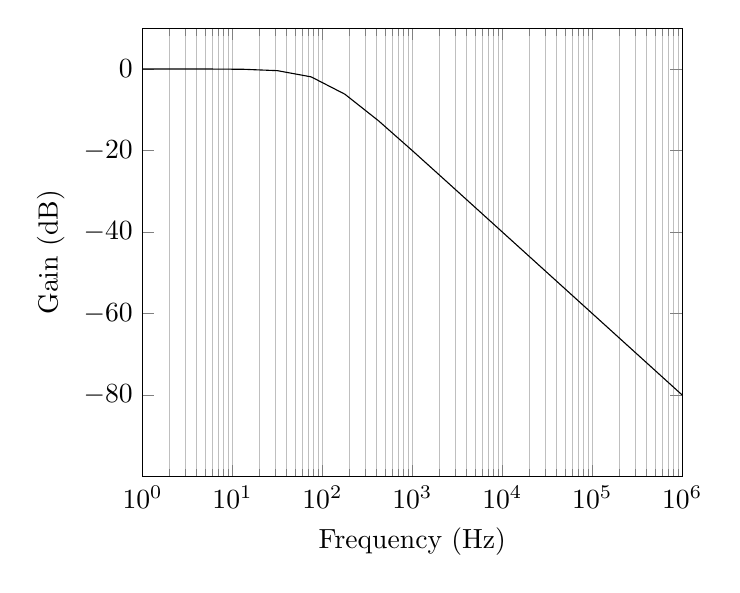
\begin{tikzpicture}
		\begin{semilogxaxis}[xmin=1, xmax=1e6, xlabel=Frequency (Hz), ymin=-100, ymax=10, ylabel=Gain (dB), ytick={0, -20, -40, -60, -80}, grid=minor]
			\addplot[domain=1:1e9]{-10*log10(1+(x/100)^2)};
		\end{semilogxaxis}
	\end{tikzpicture}
	\caption{Bode plot of the frequency response of an RC low-pass at \SI{100}{\hertz}.}\label{fig:bode_filter_rc}
\end{figure}
We can see how the frequency response suppresses frequency above \SI{100}{\hertz}.
However, efficient frequency suppression starts at \SI{-80}{\decibel} which the given RC low-pass of \Cref{fig:bode_filter_rc} only satisfies for much higher frequencies than the pole frequency.

% TODO: give example of two pole filter and how to choose parameters
One approach to improve the frequency response of a filter is to introduce additional frequency poles.
In the limit of infinite many frequency poles, one is able to approach an ideal brick-wall filter.
The frequency response of an ideal brick-wall filter resembles a step function.
In practice, one finds good enough results for two pole filters.

% TODO: give example of capacitance multiplier and how to choose parameters
In addition to a multi-pole filter, a capacitance multiplier can be used to increase the effective capacitance of a filter.
The capacitance multiplier is described in Ref.~\cite[p.~536]{Hobbs11} and Ref.~\cite[p.~578]{Horowitz15}.

\subsection{Voltage regulator}

We use two voltage regulator to maintain a constant voltage of \SI{\pm12}{\volt} which is used to supply the operational amplifiers.

In general, one needs to decide between linear and switching voltage regulators.
Linear voltage regulators are less efficient than their switching counterparts but have better noise characteristics.
As efficiency is not a concern in our application, the better noise characteristics are a strong argument for the linear voltage regulators.
Linear voltage regulators require an input voltage greater than the output voltage.
The difference between input and output voltage is called the drop-out voltage.
The drop-out voltage is about \SIrange{2}{3}{\volt}

Linear voltage regulators are available with fixed and adjustable output voltage.
As we might need an additional voltage drop between the input voltage and the voltage regulator input, e.g. for input power filters, an adjustable voltage regulator would allow for more flexibility.
Moreover, we found the range of negative voltage regulators to be rather limited.

% TODO: working principle (how does R1, R2 on the adjustable terminal change the output voltage?)
\begin{figure}[H]
	\centering
	\begin{circuitikz}
		\draw (0, 0) node[vcc, rotate=90, label={[label distance=6]:\SI[retain-explicit-plus]{+15}{\volt}}]{} -- ++(1, 0) node(node1a)[circ]{} -- ++(4, 0) node(node1b)[circ]{} -- ++(0, 2) to[diode, l_=D1] ++(-4, 0) -- ++(0, -2);
		\draw (node1b) to[resistor, l_=R1, a^=\SI{120}{\ohm}] ++(0, -2) node(node2a)[circ]{} -- ++(-2, 0) -- ++(0, 2);
		\draw (node2a) -- ++(3, 0) node(node2b)[circ]{} to[diode, l=D3] ++(0, 2) node(node1c)[circ]{} -- ++(-3 ,0);
		\draw (node1c) -- ++(2, 0) node(node1d)[circ]{} to[ecapacitor, l_=C5, a^=\SI{1}{\micro\farad}] ++(0, -4) node(node3d)[circ]{} -- ++(-2, 0) node(node3c)[circ]{} -- ++(-3, 0) node(node3b)[circ]{} to[resistor, l^=R2, a_=\SI{980}{\ohm}] ++(0, 2);
		\draw (node2b) to[ecapacitor, l_=C3, a^=\SI{10}{\micro\farad}] (node3c);
		\draw (node1d) -- ++(1, 0) node[vcc, rotate=270, label={[label distance=6]:\SI[retain-explicit-plus]{+12}{\volt}}]{};
		\begin{scope}[xshift=3cm]
			\node[draw, rectangle, fill=white, minimum width=2cm, minimum height=1.2cm, label=U1]{};
			\node at (0, 0) {LM317};
		\end{scope}
		\draw (node3d) -- ++(1, 0) node[ground, rotate=90]{};
		\draw (node3b) -- ++(-5, 0) node[ground, rotate=270]{};
		\draw (node1a) to[ecapacitor, l_=C1, a^=\SI{100}{\nano\farad}] ++(0, -4) node(node3a)[circ]{};
		\draw (node3a) to[ecapacitor, l_=C2, a^=\SI{100}{\nano\farad}] ++(0, -4) node(node5a)[circ]{};
		\draw (node5a) -- ++(-1, 0) node[vee, rotate=270, label={[label distance=6]:\SI{-15}{\volt}}]{};
		\draw (node3b) to[resistor, l_=R3, a^=\SI{980}{\ohm}] ++(0, -2) node(node4b)[circ]{} to[resistor, l_=R4, a^=\SI{120}{\ohm}] ++(0, -2) node(node5b)[circ]{} -- (node5a);
		\draw (node3c) to[ecapacitor, l_=C4, a^=\SI{10}{\micro\farad}] ++(0, -2) node(node4c)[circ]{} to[diode, l_=D4] ++(0, -2) node(node5c)[circ]{} -- (node5b);
		\draw (node3d) to[ecapacitor, l_=C6, a^=\SI{1}{\micro\farad}] ++(0, -4) node(node5d)[circ]{} -- (node5c);
		\draw (node5d) -- ++(1, 0) node[vee, rotate=90, label={[label distance=6]:\SI{-12}{\volt}}]{};
		\draw (node5a) ++(2, 0) -- ++(0, 2) -- (node4b) -- (node4c);
		\begin{scope}[xshift=3cm, yshift=-8cm]
			\node[draw, rectangle, fill=white, minimum width=2cm, minimum height=1.2cm, label=below:U2]{};
			\node at (0, 0) {LM337};
		\end{scope}
		\draw (node5b) -- ++(0, -2) to[diode, l^=D2] ++(-4, 0) -- ++(0, 2);
	\end{circuitikz}
	\caption{Dual supply voltage regulator.}\label{fig:voltage_regulator_dual}
\end{figure}
\Cref{fig:voltage_regulator_dual} illustrates the schematic of the final dual voltage regulator supply circuit.
The input voltage is buffered by capacitors C1 and C2.
U1 and U2 denote the fixed positive and negative voltage regulators.
Resistors R1 and R2 configure the output voltage of U1 to about \SI[retain-explicit-plus]{+11.5}{\volt}.
Resistors R3 and R4 configure the output voltage of U2 to about \SI[retain-explicit-plus]{-11.5}{\volt}.
Capacitors C3, C4, C5 and C6 buffer the output voltage.
When the supply power is switched off and C3 or C5 discharges,
diodes D3 and D1 redirect the current back to the supply lines around the voltage regulators.

\subsection{Voltage reference}

A voltage reference is a high-precision linear (fixed) voltage regulator.
We use it as a voltage source for the sensible reverse bias voltage of the photodiode.
\begin{figure}[H]
	\centering
	\begin{circuitikz}
		\draw (0, 0) node[vcc, rotate=90, label={[label distance=6]:\SI{15}{\volt}}]{} -- ++(1, 0) node(node1a)[circ]{} to[capacitor, l_=C1, a^=\SI{1}{\micro\farad}] ++(0, -4) node(node2a)[circ]{} -- ++(-1, 0) node[ground, rotate=270]{};
		\draw (node1a) -- ++(2, 0) node(node1b)[circ]{} -- ++(0, -4) node(node2b)[circ]{} -- (node2a);
		\draw (node1b) -- ++(2, 0) node(node1c)[circ]{} to[capacitor, l_=C2, a^=\SI{1}{\micro\farad}] ++(0, -4) node(node2c)[circ]{} -- (node2a);
		\draw (node1c) -- ++(2, 0) node(node1d)[circ]{} to[resistor, l_=R1, a^=\SI{100}{\ohm}] ++(0, -2) to[capacitor, l_=C3, a^=\SI{10}{\nano\farad}] ++(0, -2) node(node2d)[circ]{} -- (node2c);
		\draw (node1d) -- ++(2, 0) node(node1e)[circ]{} to[ecapacitor, l_=C4, a^=\SI{22}{\micro\farad}] ++(0, -4) node(node2e)[circ]{} -- (node2c);
		\draw (node1e) -- ++(1, 0) node[vcc, rotate=270, label={[label distance=6]:\SI{10}{\volt}}]{};
		\draw (node2e) -- ++(1, 0) node[ground, rotate=90]{};
		% TODO: use dipchip node and name IC ports
		\begin{scope}[xshift=4cm]
			\node[draw, rectangle, fill=white, minimum width=3cm, minimum height=1.4cm, label=above:U1]{};
			\node at (0, 0) {REF5010};
		\end{scope}
	\end{circuitikz}
	\caption{High-precision voltage reference.}\label{fig:voltage_reference}
\end{figure}
\Cref{fig:voltage_reference} depicts the schematic of the voltage reference circuit.
Capacitor C1 buffers the \SI{15}{\volt} supply voltage.
According to the datasheet the trim terminal should be connected through a capacitor, C2, to ground.
Resistor R1 and capacitor C3 form a low-pass to suppress frequency components in the kHz range.
Finally, capacitor C4 buffers the output voltage.
\section{Manufacturing}

% TODO: give rough description of manufacturing steps with images

% TODO: signal processing of non-linear response Cui10
% TODO: mention current analog-to-digital-converter in a digital signal processing section

% TODO: bill of materials / component and package selection section
% TODO: pcb design section
% TODO: manufacturing section
% TODO: section for electrical and optical test setups to check functionality

\printglossaries
\printbibliography

\end{document}